\section{Outputs}
  In this penultimate section, I will share some of the outputs the project has delivered. I will use these to reflect on the different parts of the project
  each output is associated with. To do this reflection I will use the Experience, Reflect, Action (ESA) framework founded by Melanie Jasper (2003, p.2).

  \begin{figure}[H]
    \centering
    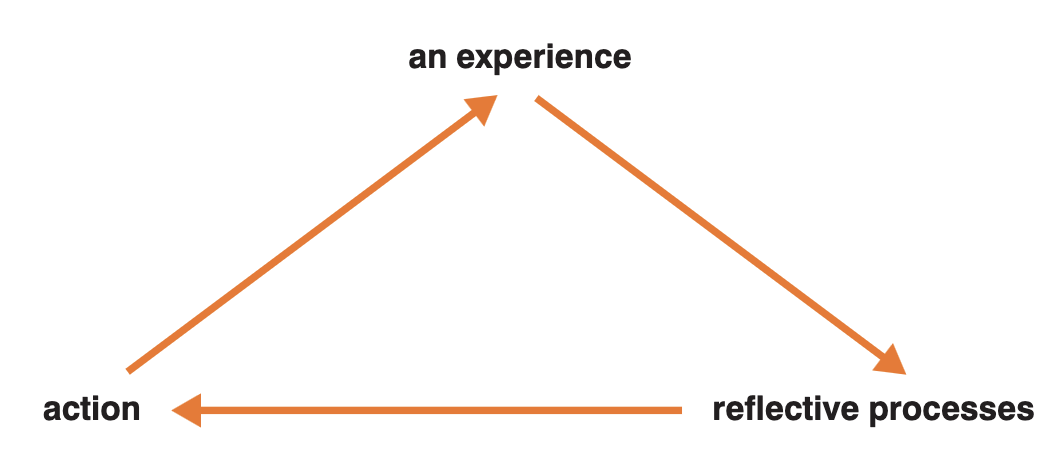
\includegraphics[width=8cm]{assets/eraReflection.png}
    \caption{ERA reflection model founded by Jasper (2003, p.2).}
    \label{fig:eraReflection}
  \end{figure}  

  \subsection{Burn-up Charts}
  \label{sec:burnup}

  \begin{figure}[H]
    \centering
    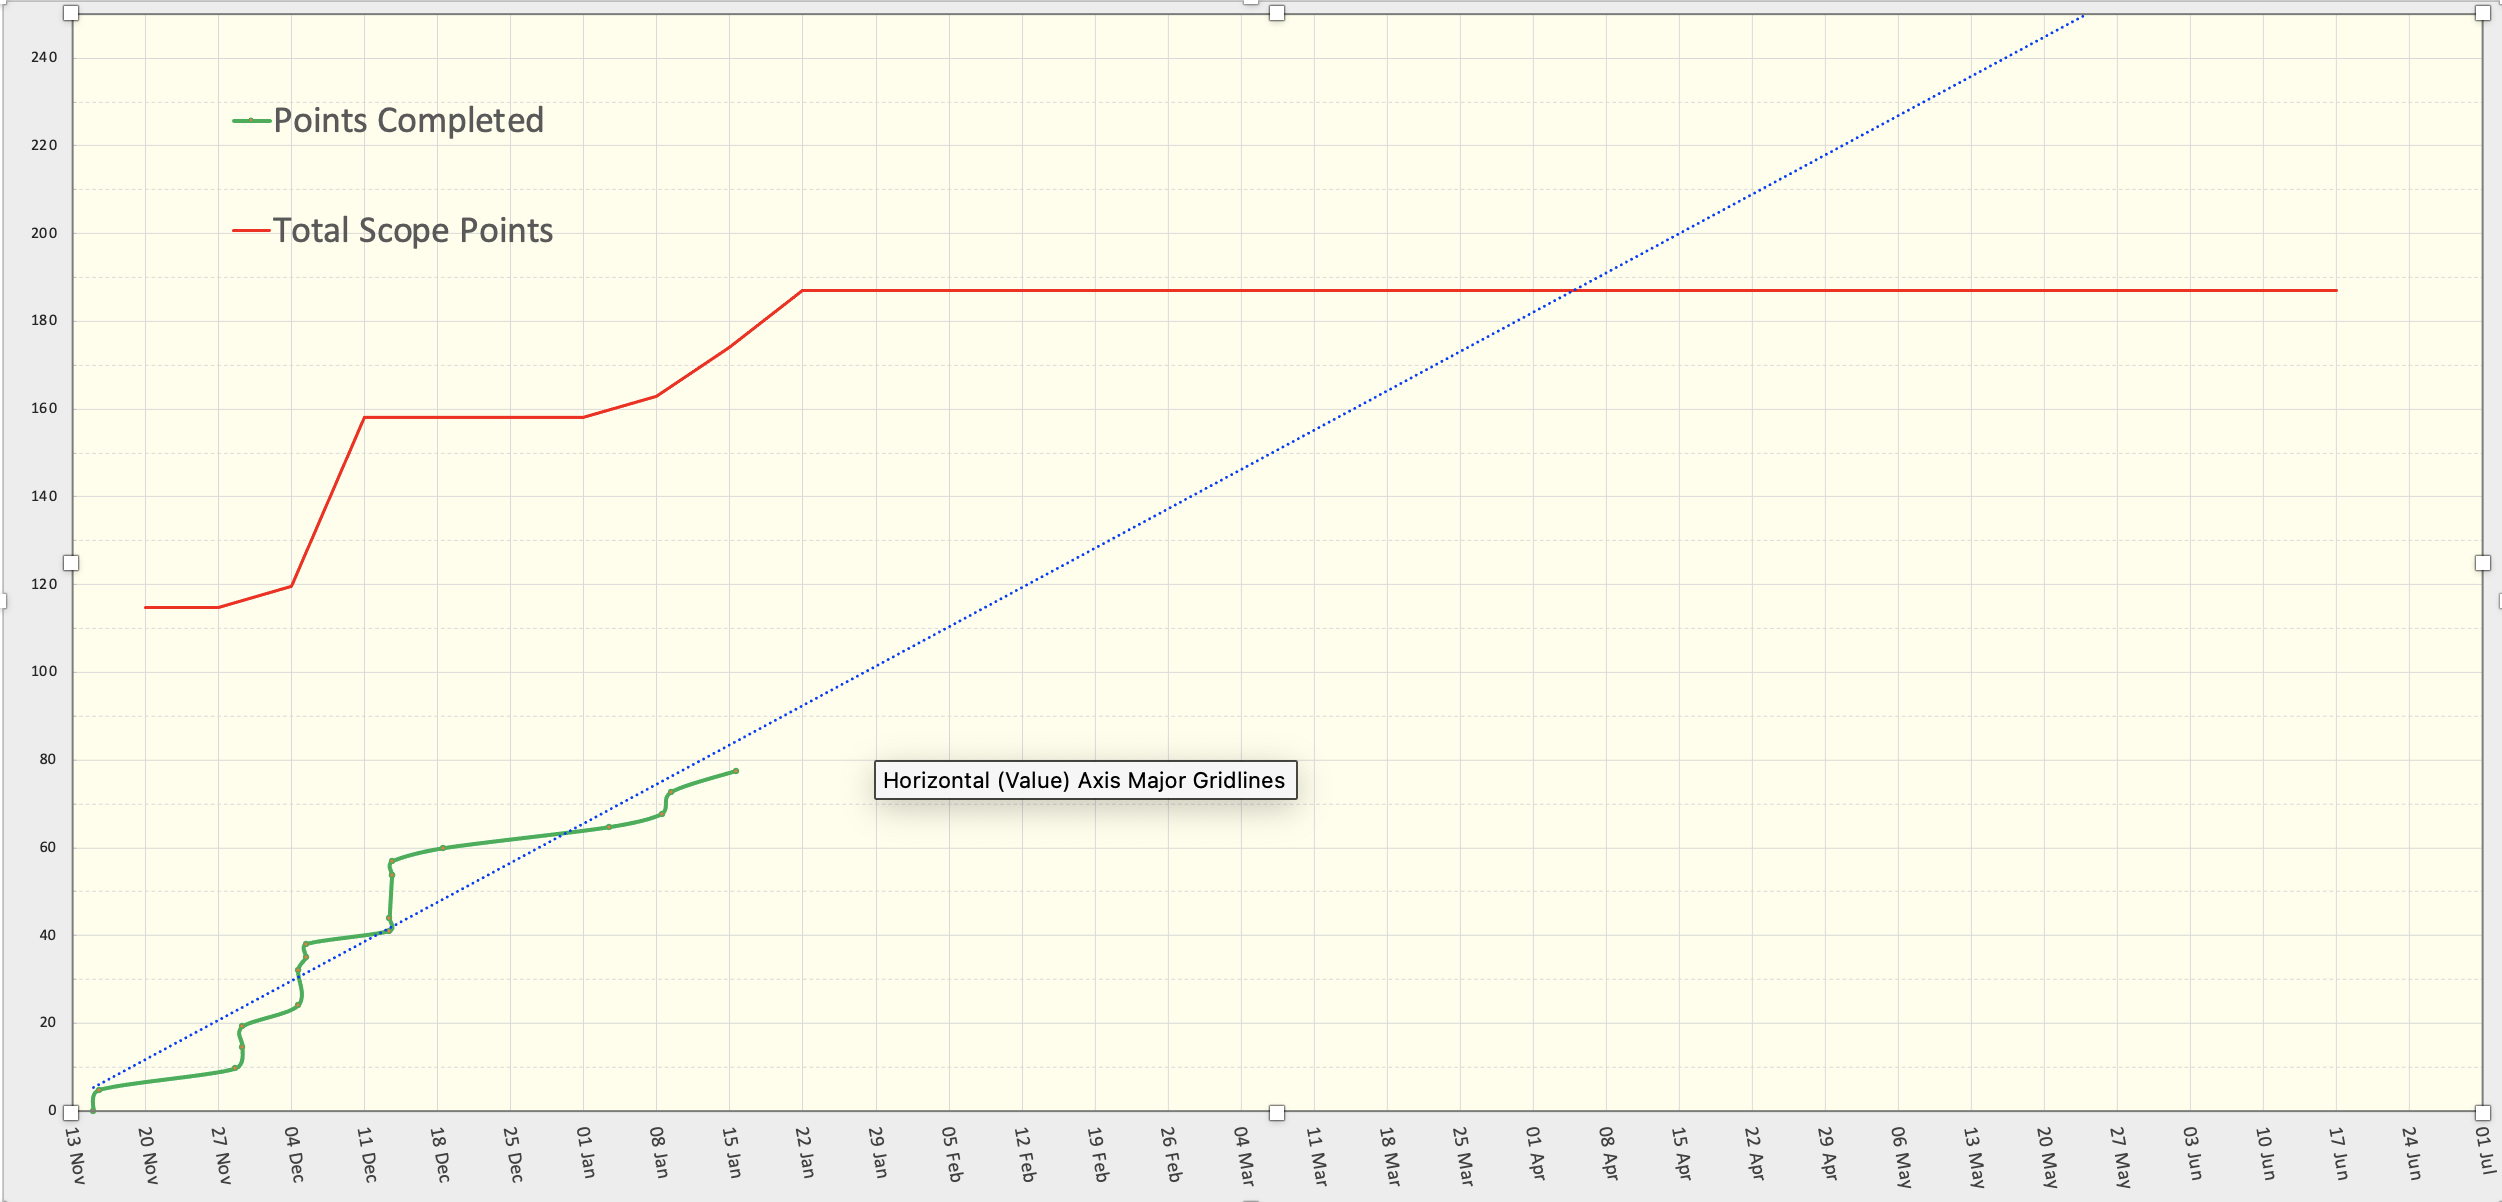
\includegraphics[width=6cm]{assets/outputs/burnups/01-16.png}
    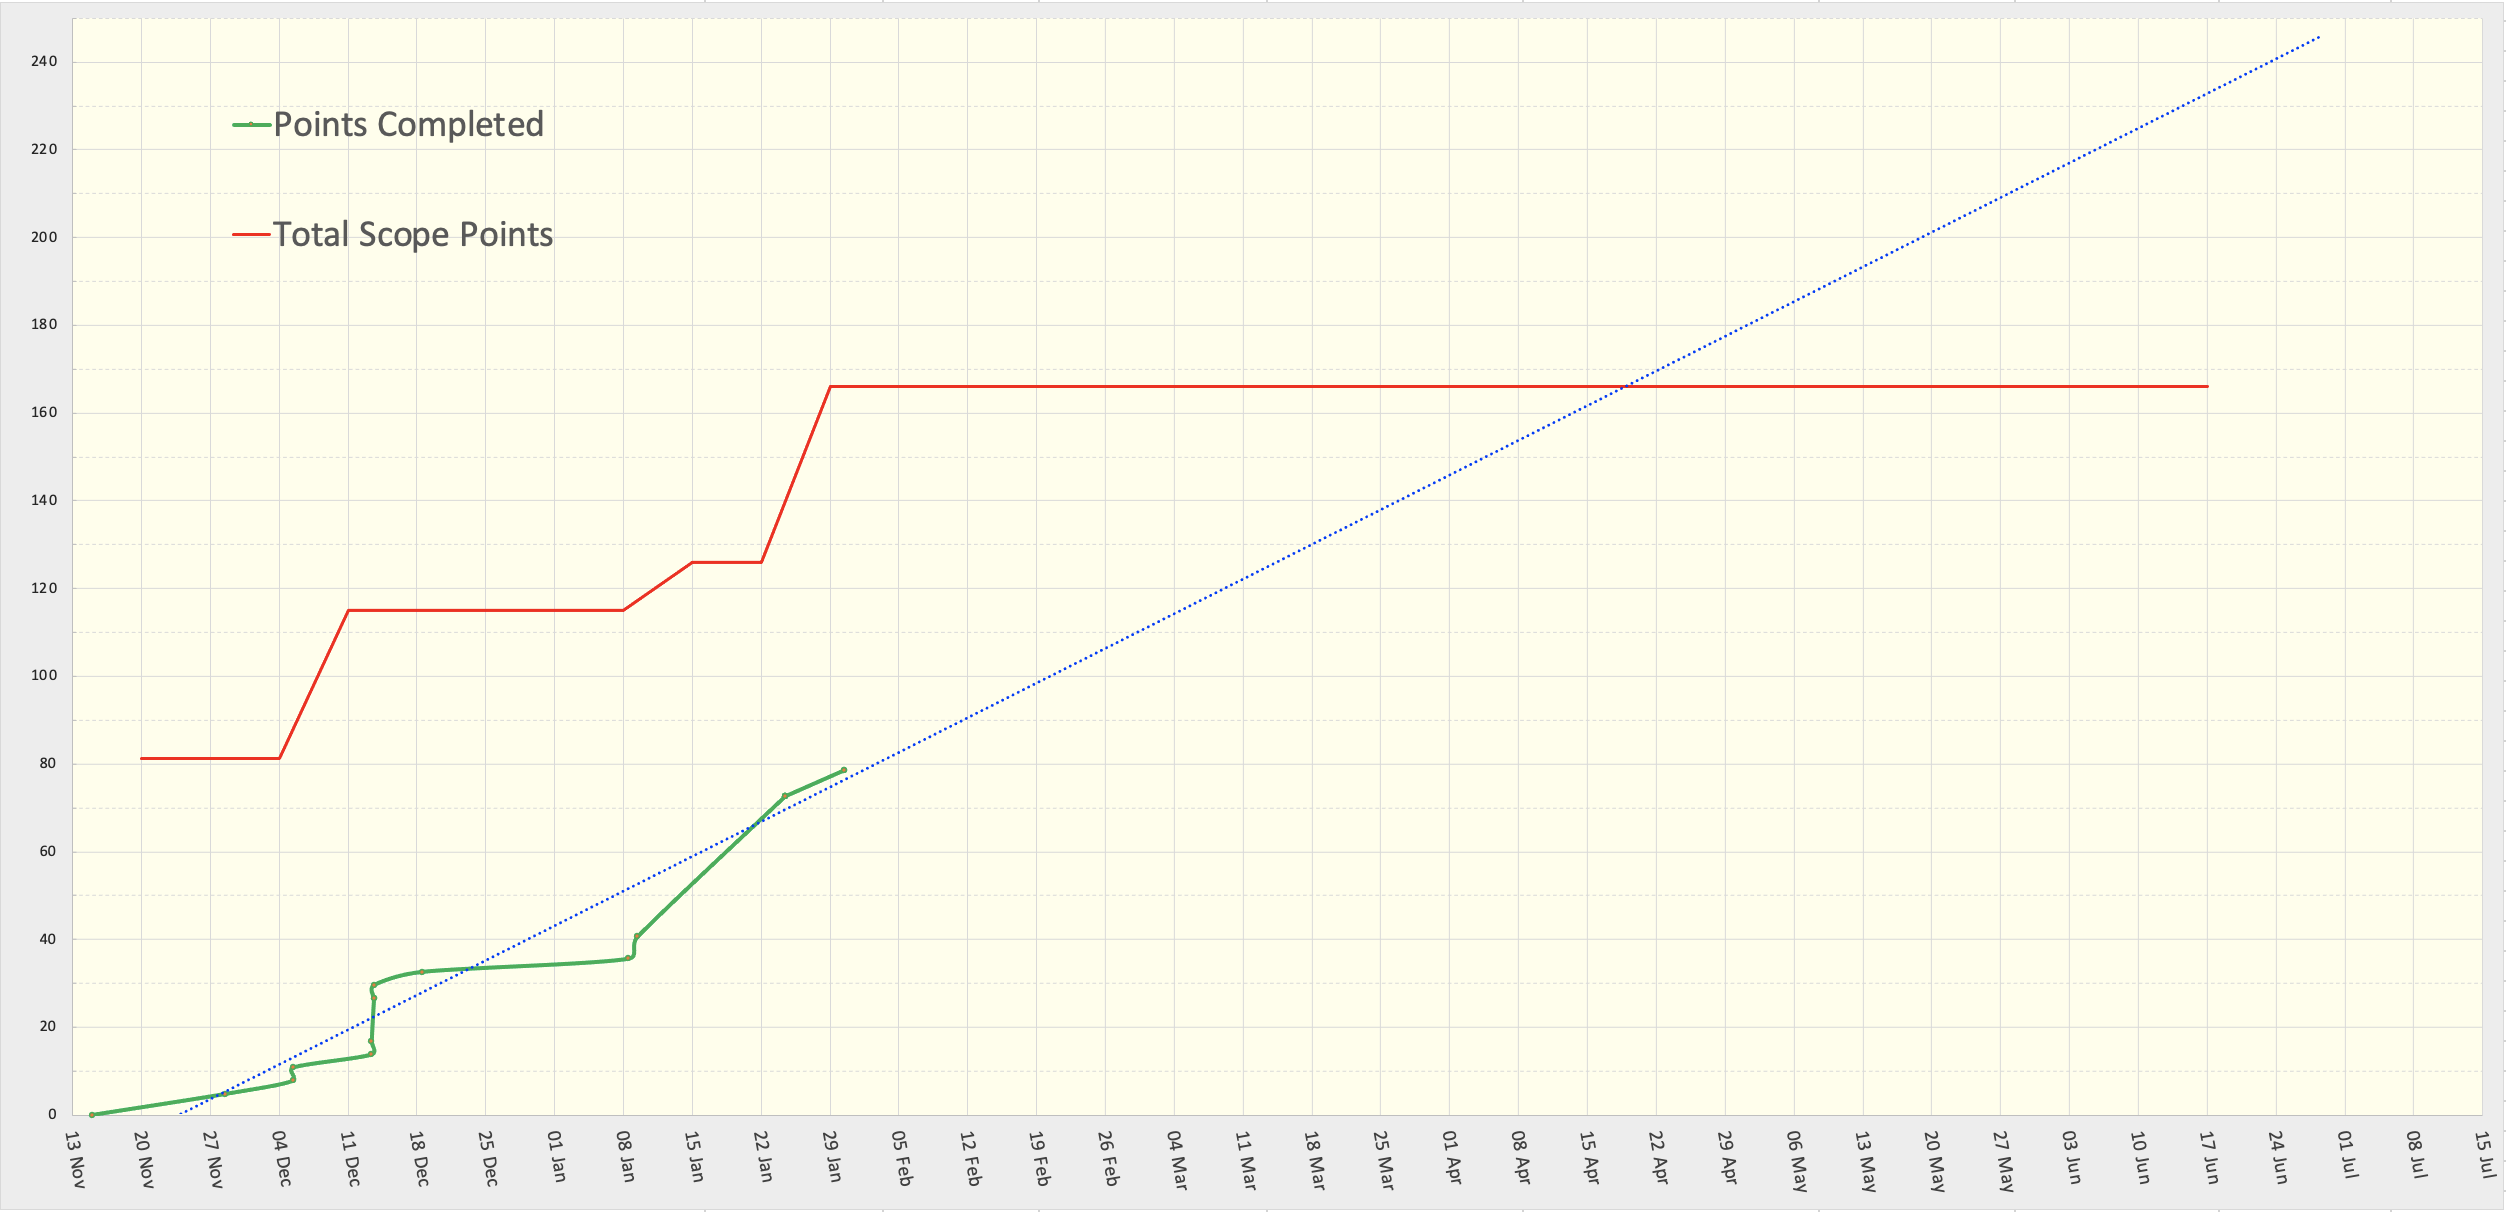
\includegraphics[width=6cm]{assets/outputs/burnups/01-30.png}
    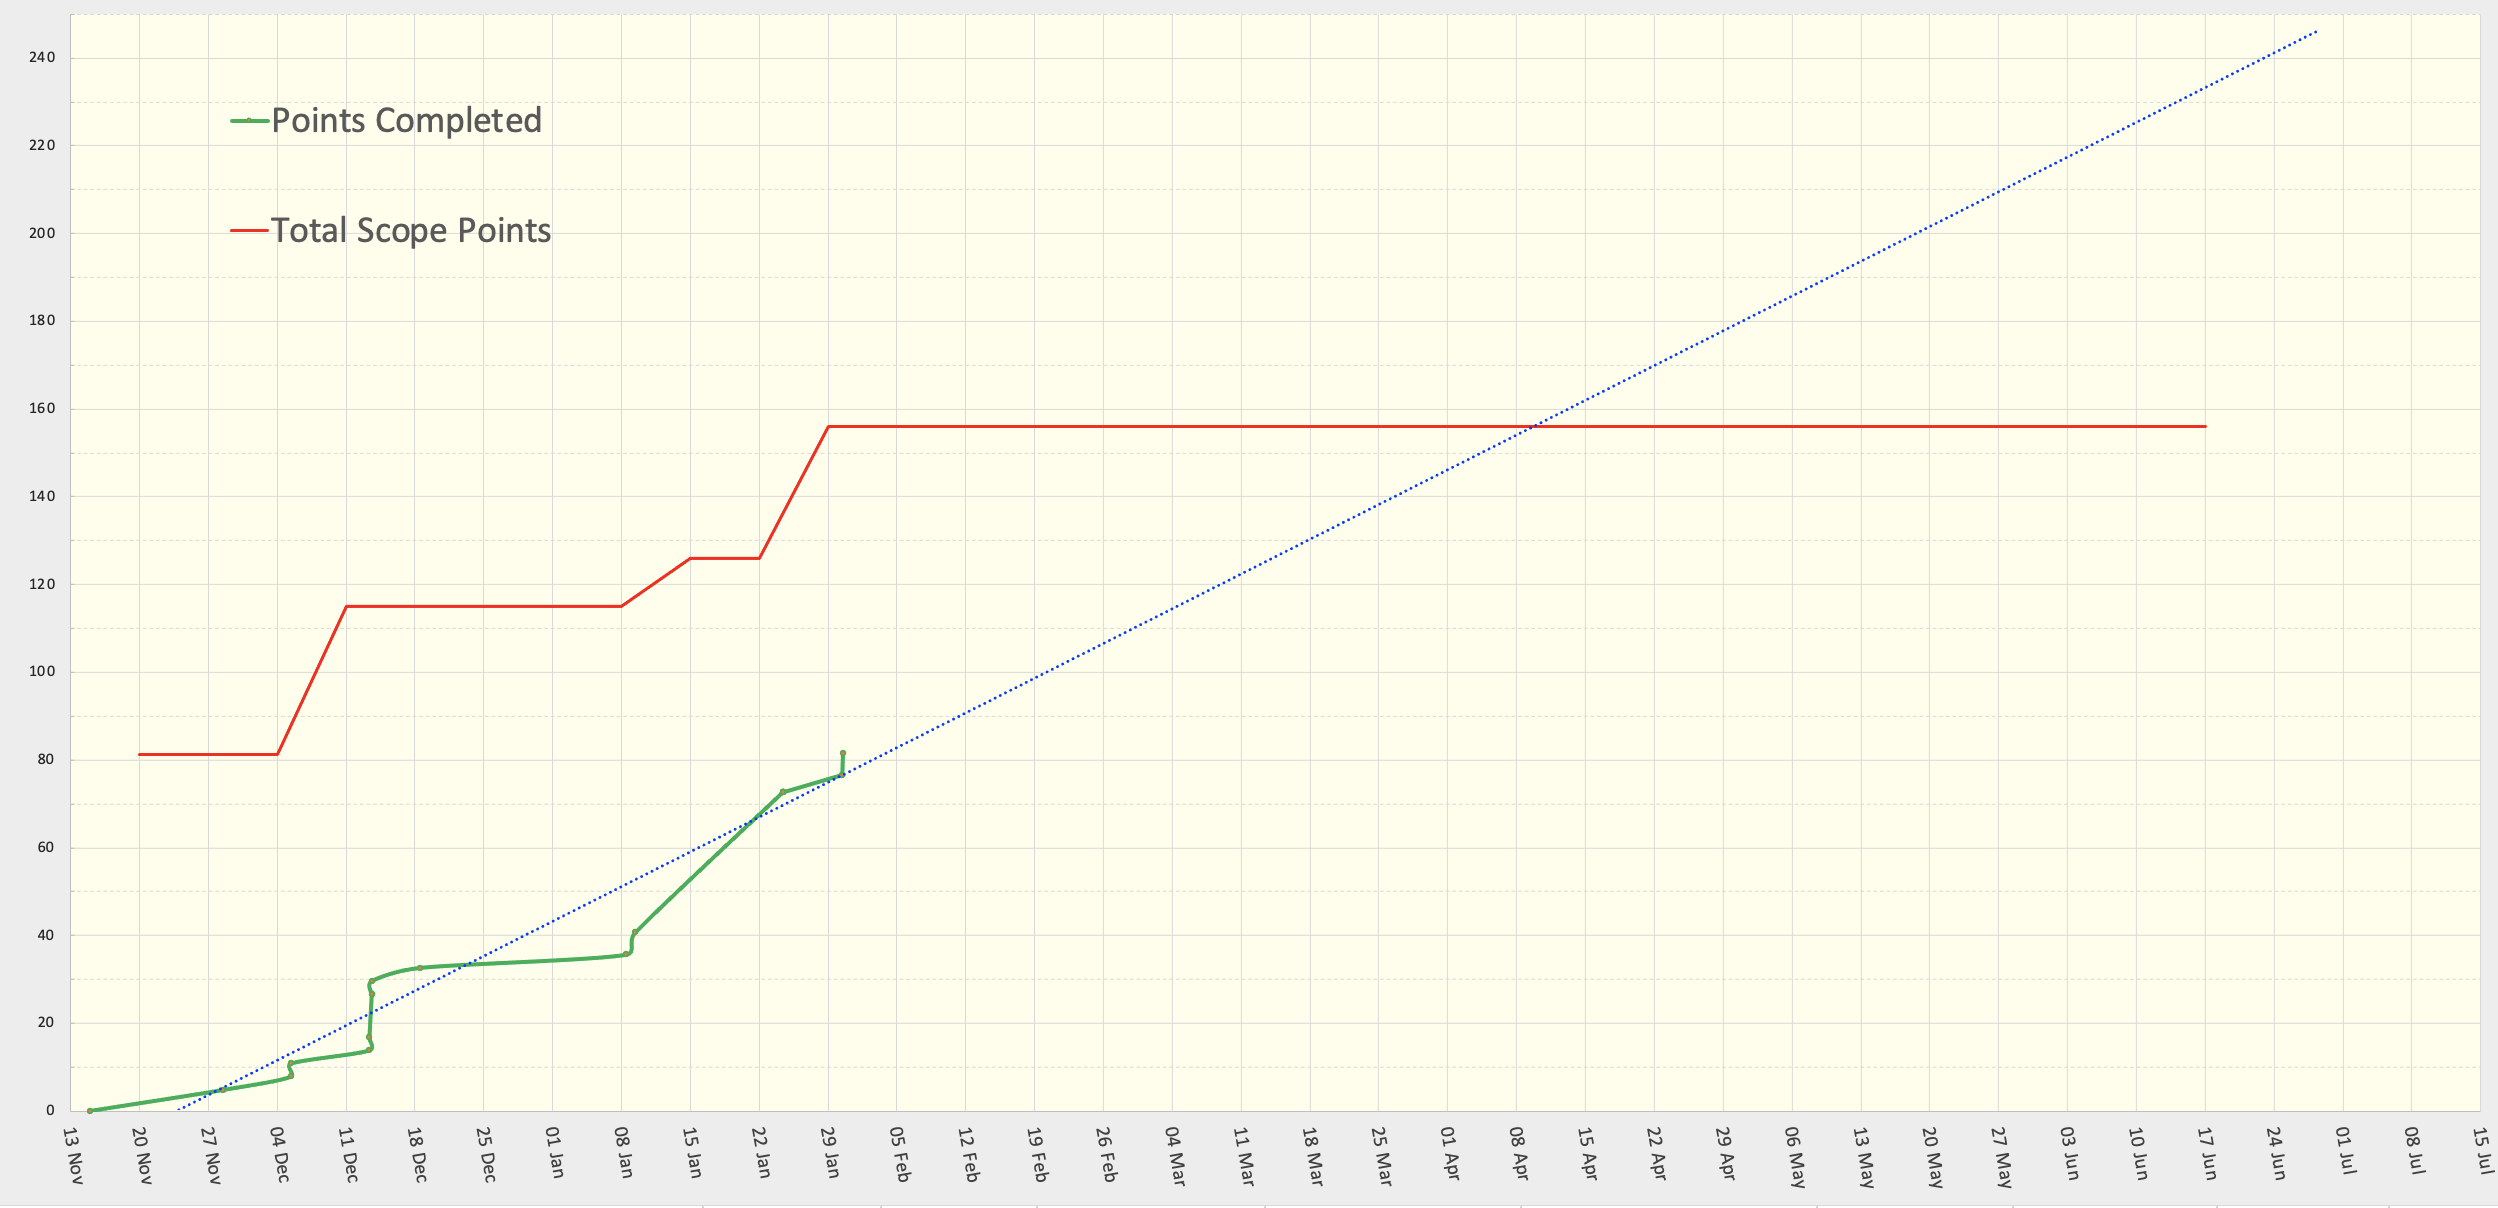
\includegraphics[width=6cm]{assets/outputs/burnups/02-05.png}
    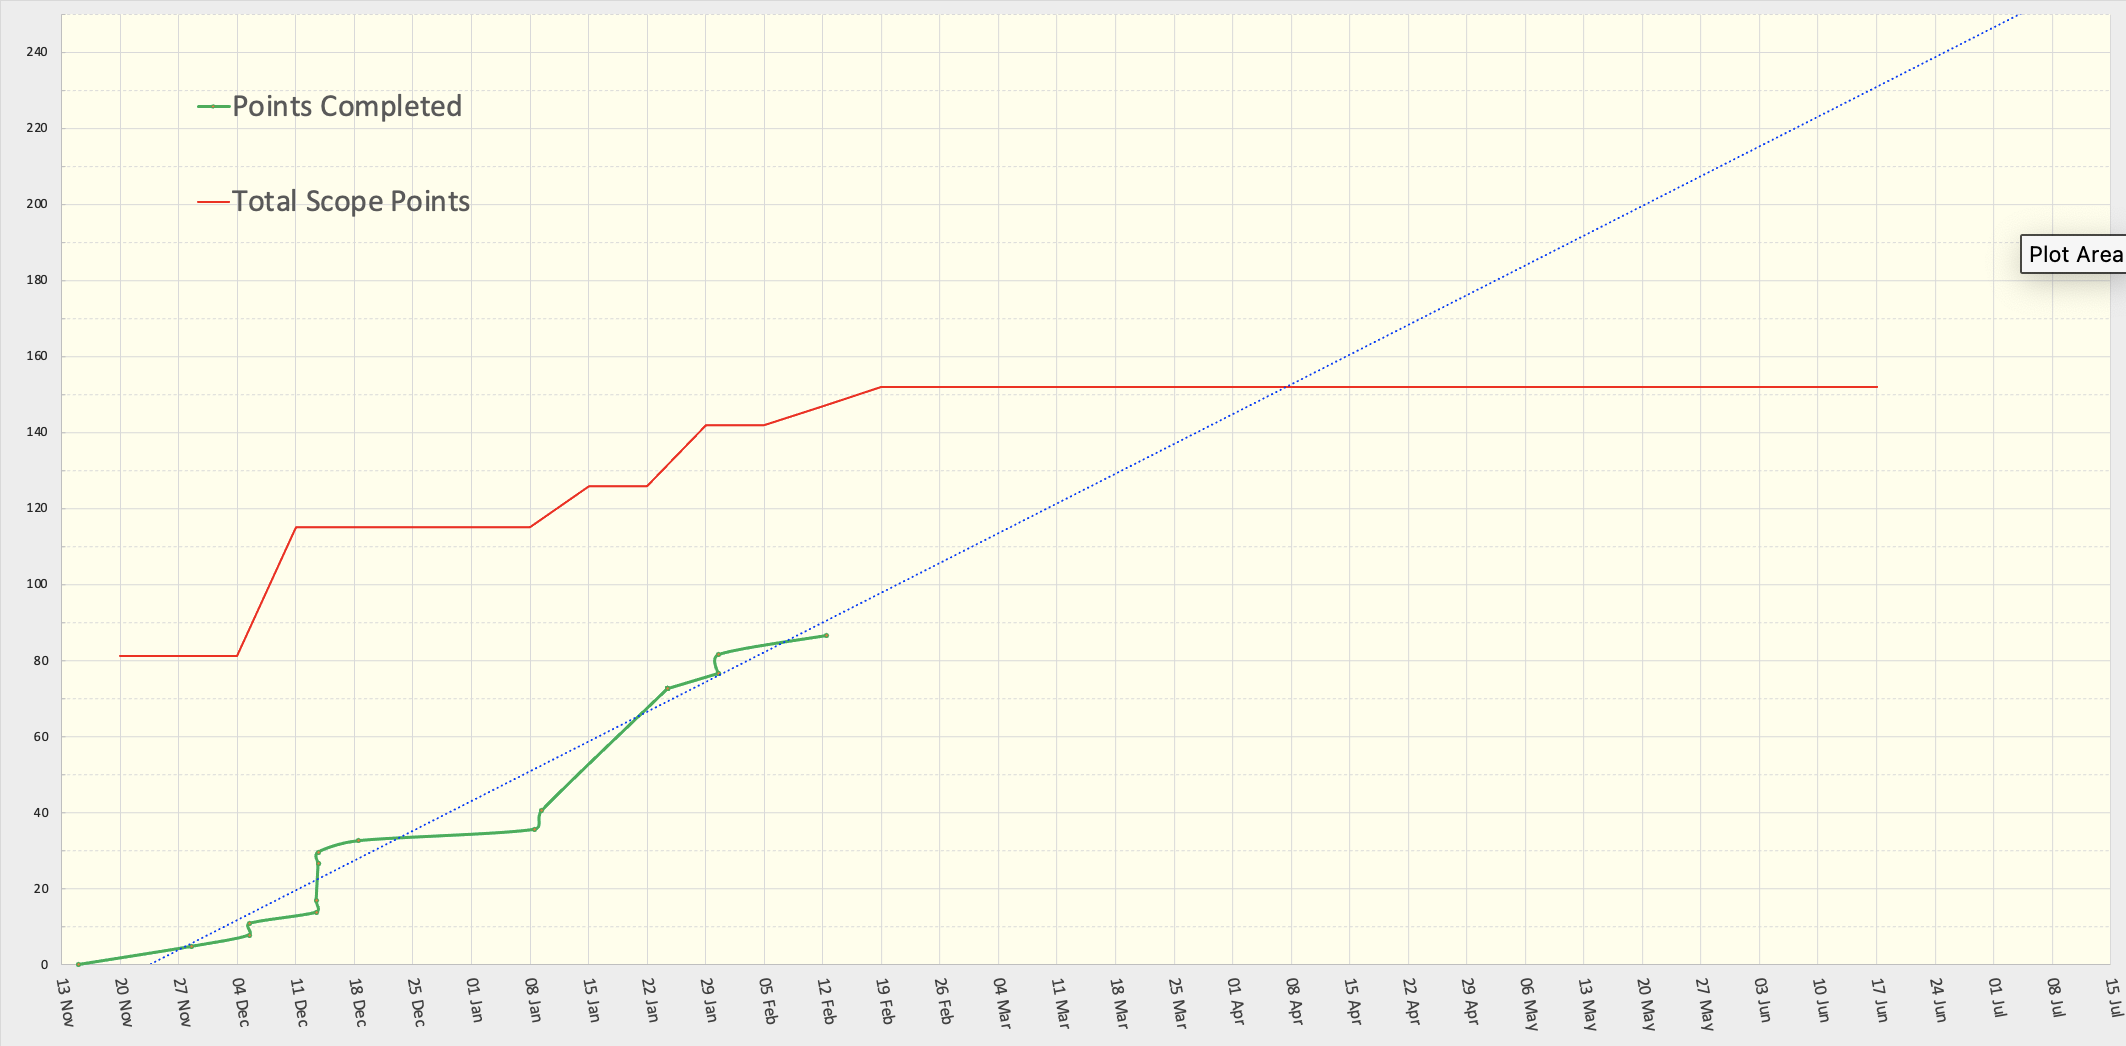
\includegraphics[width=6cm]{assets/outputs/burnups/02-14.png}
    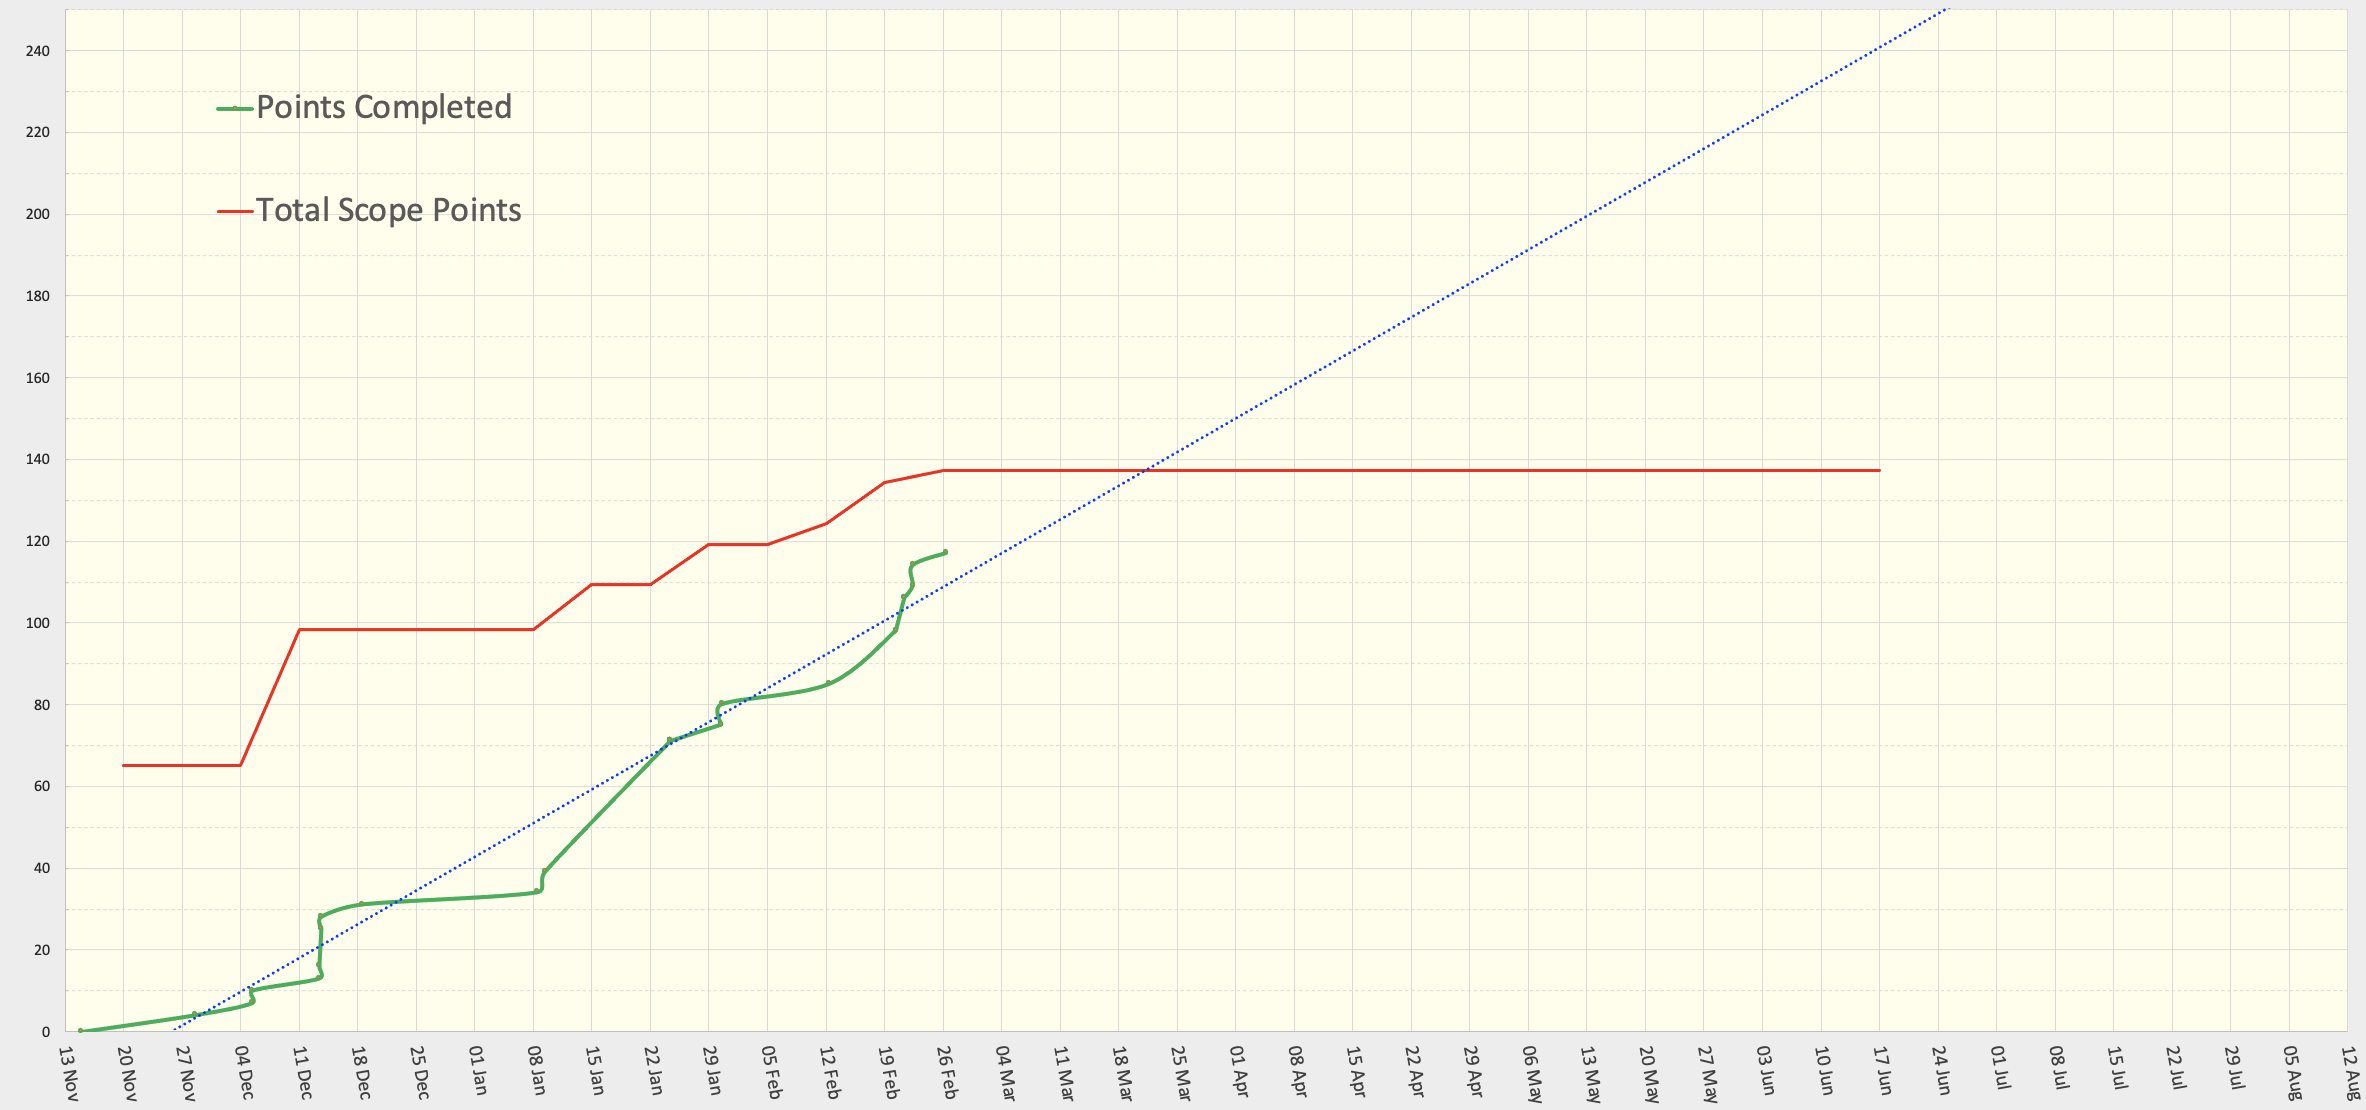
\includegraphics[width=6cm]{assets/outputs/burnups/02-27.png}
    \caption{Burn-up charts throughout the project.}
    \label{fig:burnups}
  \end{figure}

  \textbf{Experience} -
  \textbf{Reflection} -
  \textbf{Action} -

  \newpage
  \subsection{Final System Architecture}

  \begin{landscape}
    \begin{figure}[H]
      \centering
      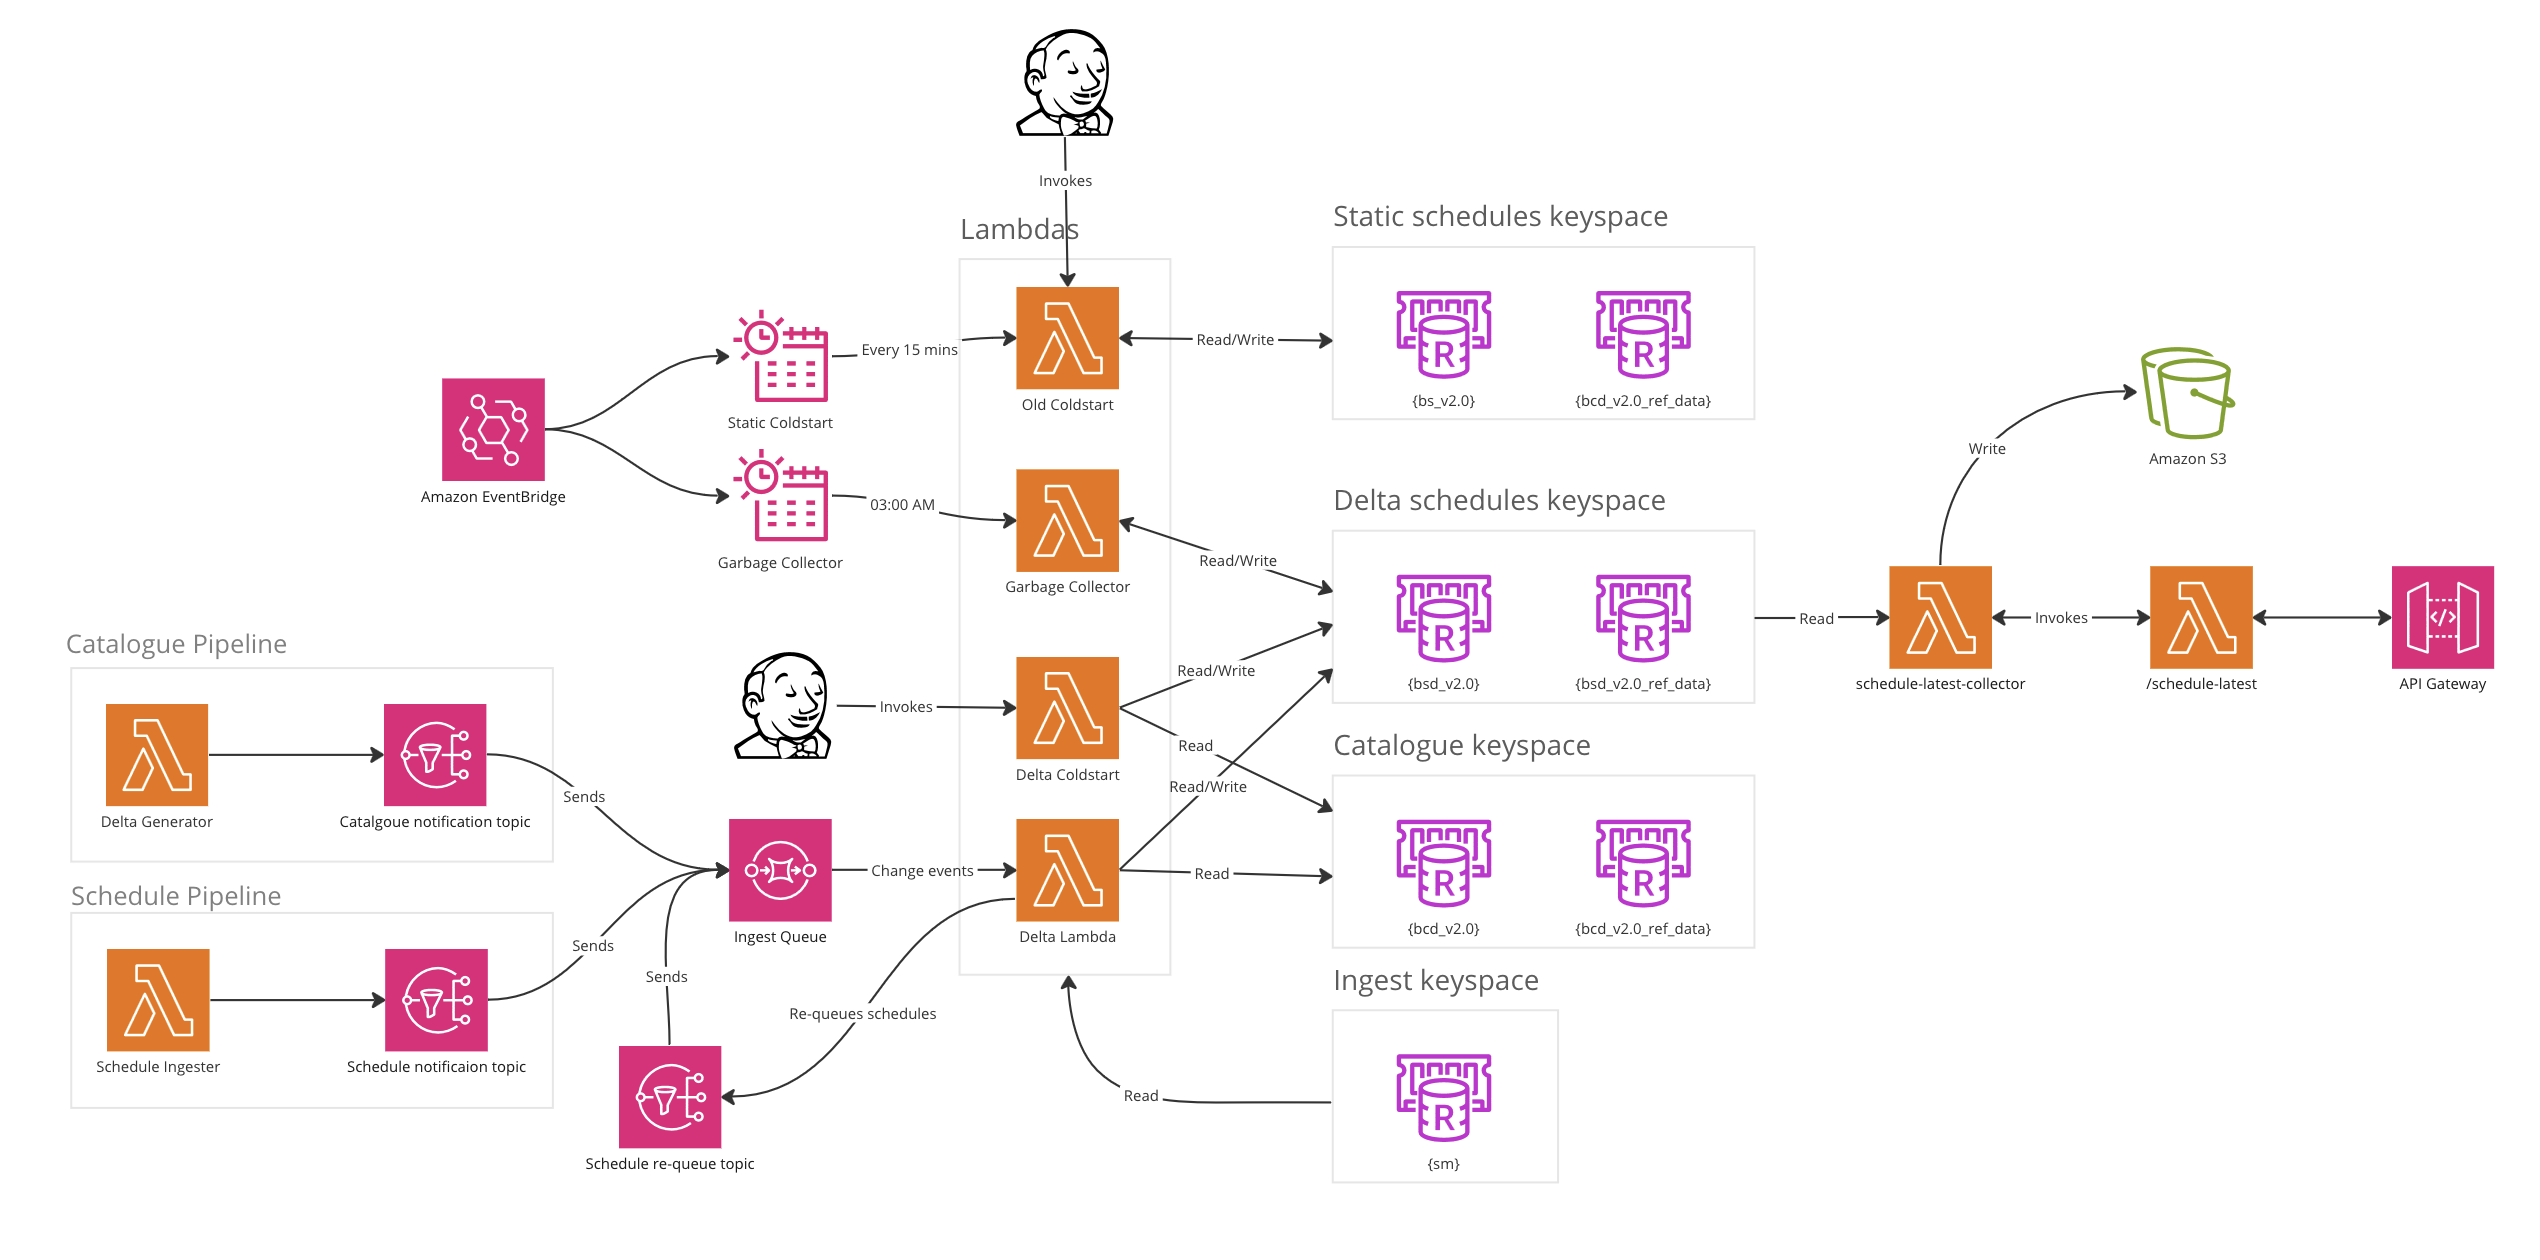
\includegraphics[width=20cm]{assets/outputs/finalArchitecture.png}
      \caption{Final architecture for project.}
      \label{fig:finalArchitecture}
    \end{figure}
  \end{landscape}

  \textbf{Experience} -
  \textbf{Reflection} -
  \textbf{Action} -

  \newpage
  \subsection{Dashboard}

  \begin{figure}[H]
    \centering
    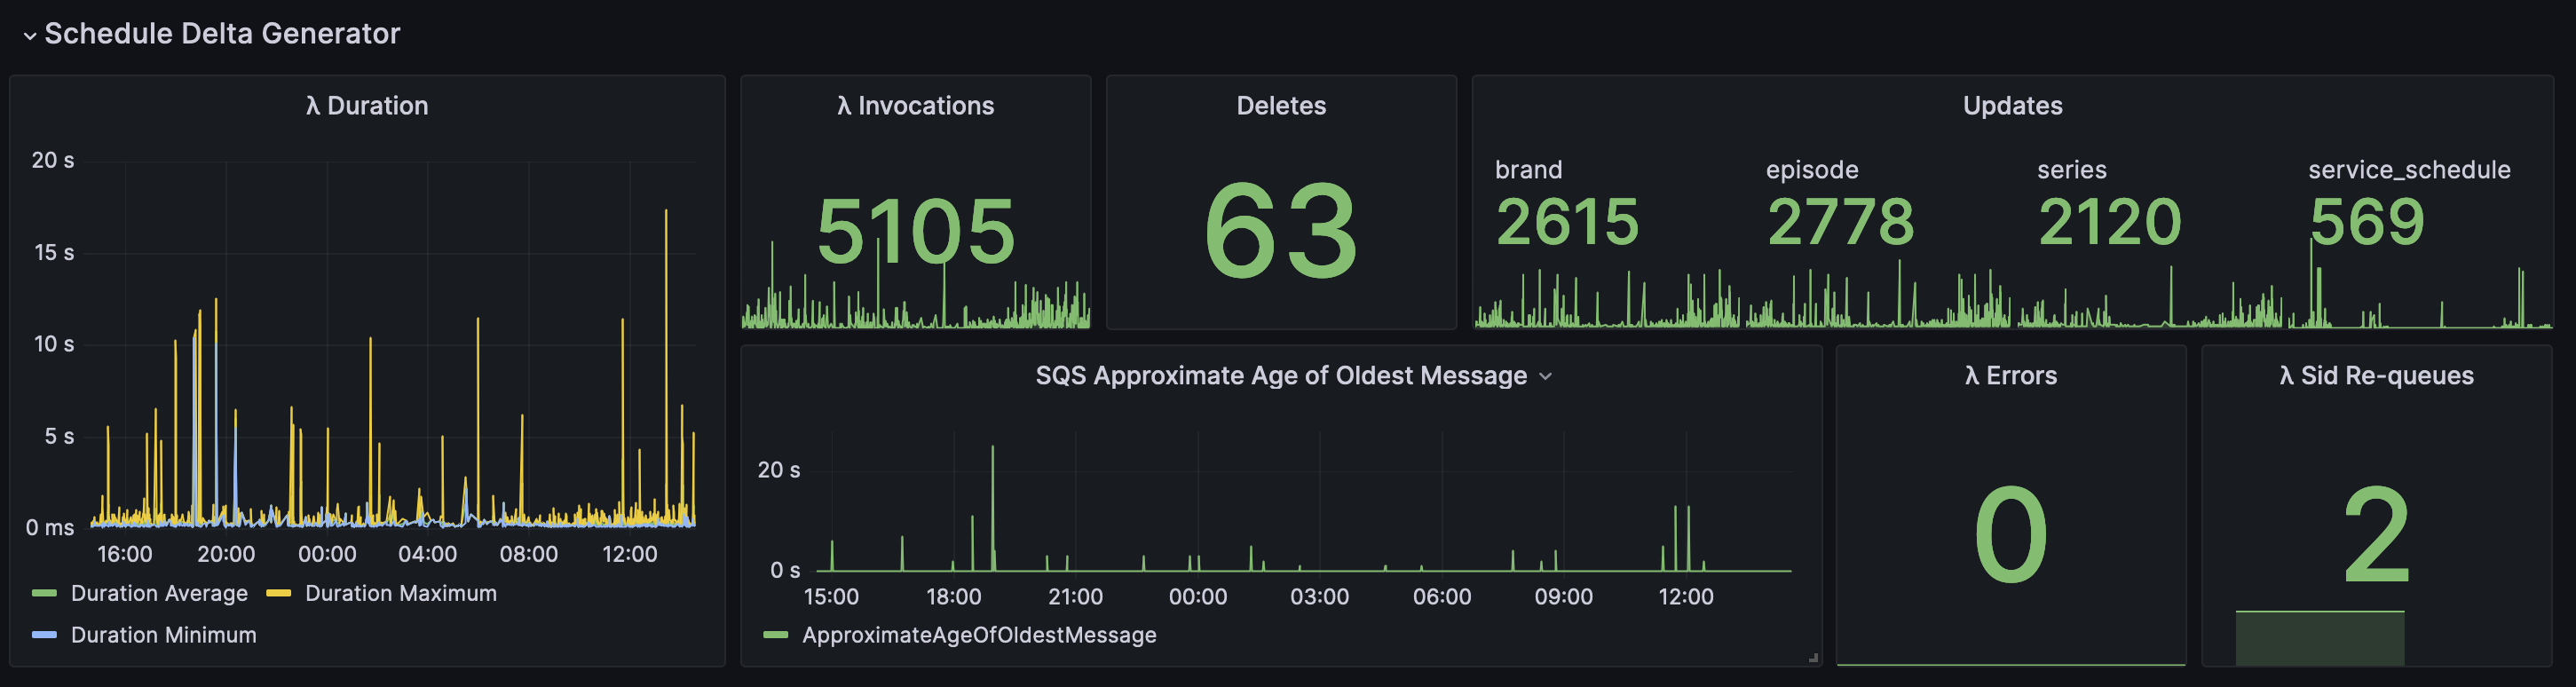
\includegraphics[width=10cm]{assets/outputs/dashboard.png}
    \caption{Created dashboard in Grafana (2024).}
    \label{fig:dashboard}
  \end{figure}

  \textbf{Experience} -
  \textbf{Reflection} -
  \textbf{Action} -
  
  \newpage
  \subsection{Code Base and Commits}

  \begin{figure}[H]
    \centering
    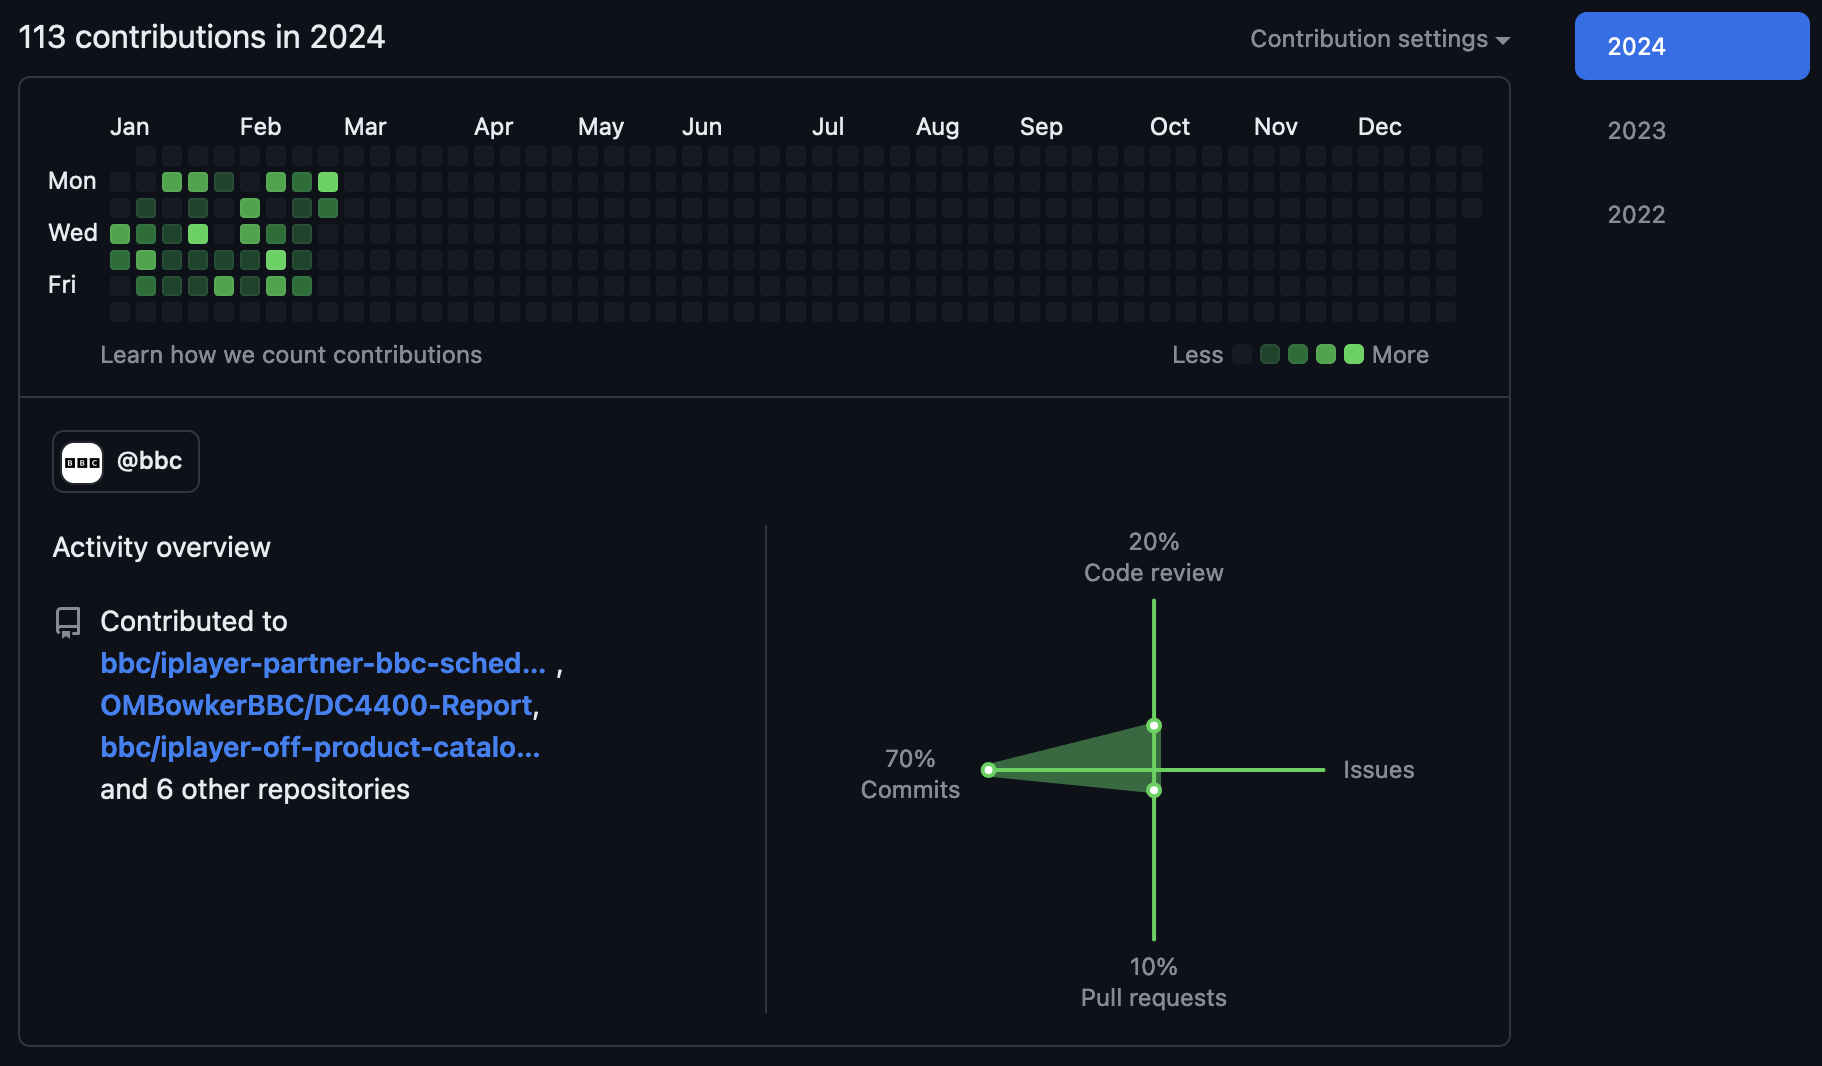
\includegraphics[width=10cm]{assets/outputs/githubContributions.png}
    \caption{Github contributions for my work profile.}
    \label{fig:githubContributions}
  \end{figure}

  \textbf{Experience} -
  \textbf{Reflection} -
  \textbf{Action} -

\newpage
